\begin{comment}
\documentclass[10pt]{article}
\usepackage{fullpage, graphicx, url}
\setlength{\parskip}{1ex}
\setlength{\parindent}{0ex}
\title{GEN08}
\begin{document}


\begin{tabular}{ccc}
The Alternative Csound Reference Manual & & \\
Previous & &Next

\end{tabular}

%\hline 
\end{comment}
\section{GEN08}
GEN08�--� Generate a piecewise cubic spline curve. \subsection*{Description}


  This subroutine will generate a piecewise cubic spline curve, the smoothest possible through all specified points. 
\subsection*{Syntax}


 \textbf{f}
 \# time size 8 a n1 b n2 c n3 d ...
\subsection*{Initialization}


 \emph{size}
 -- number of points in the table. Must be a power of 2 or power-of-2 plus 1 (see \emph{f statement}
). 


 \emph{a, b, c,}
 etc. -- ordinate values of the function. 


 \emph{n1, n2, n3 ... }
 -- length of each segment measured in stored values. May not be zero, but may be fractional. A particular segment may or may not actually store any values; stored values will be generated at integral points from the beginning of the function. The sum \emph{n1}
 + \emph{n2}
 + ... will normally equal \emph{size}
 for fully specified functions. 


 


\begin{tabular}{cc}
\textbf{Note}
 \\
� &

 


 
\begin{itemize}
\item 

 \emph{GEN08}
 constructs a stored table from segments of cubic polynomial functions. Each segment runs between two specified points but depends as well on their neighbors on each side. Neighboring segments will agree in both value and slope at their common point. (The common slope is that of a parabola through that point and its two neighbors). The slope at the two ends of the function is constrained to be zero (flat). 

\item 

 \emph{Hint:}
 to make a discontinuity in slope or value in the function as stored, arrange a series of points in the interval between two stored values; likewise for a non-zero boundary slope. 


\end{itemize}


\end{tabular}

\subsection*{Examples}


  Here is a simple example of the GEN08 routine. It uses the files \emph{gen08.orc}
 and \emph{gen08.sco}
. It will create a curve with a smooth hump in the middle, going briefly negative outside the hump then flat at its ends. Here is its diagram: 


 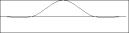
\includegraphics[scale=1]{gen08} 


 Diagram of the waveform generated by GEN08.


 \textbf{Example 1. A simple example of the GEN08 routine.}

\begin{lstlisting}
/* gen08.orc */
; Initialize the global variables.
sr = 44100
kr = 4410
ksmps = 10
nchnls = 1

; Instrument #1.
instr 1
  ; Create an index over the length of our entire note.
  kcps init 1/p3
  kndx phasor kcps

  ; Read Table #1 with our index.
  ifn = 1
  ixmode = 1
  kval table kndx, ifn, ixmode

  ; Generate a sine waveform, use our Table #1 value to 
  ; vary its frequency by 100 Hz from its base frequency.
  ibasefreq = 440
  kfreq = kval * 100
  a1 oscil 20000, ibasefreq + kfreq, 2
  out a1
endin
/* gen08.orc */
        
\end{lstlisting}
\begin{lstlisting}
/* gen08.sco */
; Table #1: a curve with a smooth hump (using GEN08).
f 1 0 65 8 0 16 0 16 1 16 0 16 0
; Table #2, a sine wave.
f 2 0 16384 10 1

; Play Instrument #1 for two seconds.
i 1 0 2
e
/* gen08.sco */
        
\end{lstlisting}
\subsection*{See Also}


 \emph{GEN05}
, \emph{GEN06}
, and \emph{GEN07}

%\hline 


\begin{comment}
\begin{tabular}{lcr}
Previous &Home &Next \\
GEN07 &Up &GEN09

\end{tabular}


\end{document}
\end{comment}
